\documentclass{urdu-textbook}
\begin{document}
\begin{center}
{\color{seccolor}\Huge\bfseries طبیعیات}\\[10pt]
{\latinfont\Large University Physics (Urdu)}\\[8pt]
{\latinfont\large PHYS-101}\\[6pt]
{\latinfont\small Halliday, Resnick, Walker — selected chapters}
\end{center}
{\color{rulecolor}\rule{\linewidth}{1.2pt}}
\vspace{1.5em}
\clearpage
\TextbookChapter{1}{پیمائش}
\hypertarget{ux686ux6ccux632ux648ux6ba-ux6a9ux6cc-ux67eux6ccux645ux627ux626ux634-ux628ux634ux645ux648ux644-ux637ux648ux627ux644ux62a}{%
\section{چیزوں کی پیمائش (بشمول
طوالت)}\label{ux686ux6ccux632ux648ux6ba-ux6a9ux6cc-ux67eux6ccux645ux627ux626ux634-ux628ux634ux645ux648ux644-ux637ux648ux627ux644ux62a}}

\hypertarget{ux637ux628ux6ccux639ux6ccux627ux62a-ux6a9ux6ccux627-ux6c1ux6d2}{%
\subsection{طبیعیات کیا
ہے؟}\label{ux637ux628ux6ccux639ux6ccux627ux62a-ux6a9ux6ccux627-ux6c1ux6d2}}

سائنس اور انجینئری کی پوری عمارت پیمائش اور موازنے پر کھڑی ہے۔ کسی بھی
چیز کو ناپنے اور دوسری چیزوں سے موازنہ کرنے کے لیے ہمیں مقرر اصول اور
تجربات درکار ہوتے ہیں جن کی مدد سے اکائیاں طے کی جاتی ہیں۔ طبیعیات کا
ایک بنیادی مقصد یہی ہے کہ ایسے تجربات کی منصوبہ بندی اور انجام دہی کی
جائے۔ مثال کے طور پر، طبیعیات دان نہایت درست گھڑیاں بنانے کی کوشش کرتے
ہیں تاکہ وقت اور وقت کے وقفوں کو بڑی صحت کے ساتھ ناپا جا سکے۔ ایسی غیر
معمولی درستی واقعی اہم ہے: مثلاً جدید عالمی نظامِ مقامیابی \en{(GPS)} انتہائی
درست گھڑیوں کے بغیر بے کار ہو جائے۔

\hypertarget{ux686ux6ccux632ux648ux6ba-ux6a9ux6cc-ux67eux6ccux645ux627ux626ux634}{%
\subsection{چیزوں کی
پیمائش}\label{ux686ux6ccux632ux648ux6ba-ux6a9ux6cc-ux67eux6ccux645ux627ux626ux634}}

ہم ہر طبیعی مقدار کو اُس کی اپنی اکائی میں، کسی معیار سے موازنہ کر کے
ناپتے ہیں۔ \textbf{اکائی} وہ منفرد نام ہے جو ہم کسی مقدار کے ناپ کو دیتے
ہیں --- مثلاً طول کے لیے \textbf{میٹر}۔ \textbf{معیار} ٹھیک \(1.0\) اکائی
کے برابر ہوتا ہے۔ معیار قائم کرنے کے بعد ہمیں ایسے طریقے وضع کرنے ہوتے
ہیں جن سے ہر طوالت --- خواہ وہ کسی ہائیڈروجن ایٹم کا نصف قطر ہو، کسی
تختۂ سکیٹ کی لمبائی ہو، یا کسی ستارے تک کا فاصلہ ہو --- اسی معیار کی
اصطلاح میں بیان کی جا سکے۔

\hypertarget{ux628ux646ux6ccux627ux62fux6cc-ux645ux642ux62fux627ux631ux6ccux6ba}{%
\subsubsection{بنیادی
مقداریں}\label{ux628ux646ux6ccux627ux62fux6cc-ux645ux642ux62fux627ux631ux6ccux6ba}}

طبیعی مقداریں بے شمار ہیں، مگر یہ سب ایک دوسرے سے آزاد نہیں۔ مثلاً رفتار
محض طول اور وقت کا تناسب ہے۔ چنانچہ ہم بین الاقوامی اتفاقِ رائے سے چند
مقداروں کو --- جیسے طول اور وقت --- \textbf{بنیادی مقداریں} مقرر کر لیتے
ہیں اور صرف اِنھی کے معیار طے کرتے ہیں۔ باقی تمام (\textbf{مشتق}) مقداریں
اِنھی بنیادی مقداروں کی مدد سے بیان کی جاتی ہیں۔

بنیادی معیار کا \textbf{قابلِ رسائی} اور \textbf{ناقابلِ تبدیل} ہونا ضروری
ہے۔ اگر ہم طول کا معیار ایک شخص کی ناک سے پھیلائی ہوئی اُنگلی تک کا فاصلہ
مقرر کریں تو وہ قابلِ رسائی تو ہوگا مگر ہر شخص کے لیے مختلف ہوگا --- یعنی
ناقابلِ بھروسہ۔ اِسی لیے سائنس میں ہم اوّلاً ناقابلِ تبدیلی کو ترجیح دیتے
ہیں۔

\hypertarget{ux628ux6ccux646-ux627ux644ux627ux642ux648ux627ux645ux6cc-ux646ux638ux627ux645-ux627ux6a9ux627ux626ux6ccux627ux62a-si}{%
\subsection{بین الاقوامی نظامِ اکائیات
\en{(SI)}}\label{ux628ux6ccux646-ux627ux644ux627ux642ux648ux627ux645ux6cc-ux646ux638ux627ux645-ux627ux6a9ux627ux626ux6ccux627ux62a-si}}

سنہ \(1971\) میں وزن و پیمائش کی چودھویں عالمی کانفرنس نے سات مقداروں کو
بنیادی مقرر کیا، جن سے \textbf{بین الاقوامی نظامِ اکائیات} (مختصراً \en{SI}،
جسے عام طور پر میٹرک نظام کہا جاتا ہے) قائم ہوا۔ ذیل کی جدول اُن تین
بنیادی مقداروں کی اکائیاں دکھاتی ہے جو ابتدائی ابواب میں استعمال ہوتی
ہیں۔

\begin{longtable}[]{@{}ccc@{}}
\toprule\noalign{}
مقدار & اکائی کا نام & علامت \\
\midrule\noalign{}
\endhead
\bottomrule\noalign{}
\endlastfoot
طول & میٹر & \(\mathrm{m}\) \\
وقت & سیکنڈ & \(\mathrm{s}\) \\
کمیت & کلوگرام & \(\mathrm{kg}\) \\
\end{longtable}

جدول ۱-۱: تین بنیادی \en{SI} اکائیاں

بہت سی مشتق \en{SI} اکائیاں اِنھی بنیادی اکائیوں سے بنتی ہیں۔ مثلاً
\textbf{طاقت} \en{(power)} کی اکائی \textbf{واٹ} \en{(W)} کو کمیت، طول اور وقت کی
بنیادی اکائیوں سے یوں بیان کیا جاتا ہے:

\[1\ \mathrm{W} = 1\ \mathrm{kg\cdot m^{2}/s^{3}}.\]

\hypertarget{ux633ux627ux626ux646ux633ux6cc-ux627ux634ux627ux631ux6ccux627ux62aux6cc-ux637ux631ux6ccux642ux6c1-ux627ux648ux631-ux633ux627ux628ux642ux6d2}{%
\subsection{سائنسی اشاریاتی طریقہ اور
سابقے}\label{ux633ux627ux626ux646ux633ux6cc-ux627ux634ux627ux631ux6ccux627ux62aux6cc-ux637ux631ux6ccux642ux6c1-ux627ux648ux631-ux633ux627ux628ux642ux6d2}}

بہت بڑی یا بہت چھوٹی مقداروں کو لکھنے کے لیے ہم \textbf{سائنسی اشاریاتی
طریقہ} (دس کی قوّتوں) سے کام لیتے ہیں:

\[3\,560\,000\,000\ \mathrm{m} = 3.56\times10^{9}\ \mathrm{m},\]

\[0.000\,000\,492\ \mathrm{s} = 4.92\times10^{-7}\ \mathrm{s}.\]

کمپیوٹر پر یہی اشاریہ مختصراً \(3.56\times10^{9}\) اور
\(4.92\times10^{-7}\) لکھا جاتا ہے (کمپیوٹر شکل میں کبھی
\(3.56\mathrm{E}9\) / \(4.92\mathrm{E}{-7}\))، جہاں \en{E} کا مطلب ''دس کی
قوّت`` ہے۔

سہولت کے لیے ہم \textbf{سابقے} \en{(prefixes)} بھی استعمال کرتے ہیں۔ ہر سابقہ
دس کی ایک خاص قوّت کو ظاہر کرتا ہے، جسے ضربی عامل کے طور پر لگایا جاتا
ہے:

\[1.27\times10^{9}\ \mathrm{watt} = 1.27\ \mathrm{gigawatt} = 1.27\ \mathrm{GW}.\]

\begin{longtable}[]{@{}ccc@{}}
\toprule\noalign{}
عامل & سابقہ & علامت \\
\midrule\noalign{}
\endhead
\bottomrule\noalign{}
\endlastfoot
\(10^{24}\) & یوٹا & \(\mathrm{Y}\) \\
\(10^{21}\) & زیٹا & \(\mathrm{Z}\) \\
\(10^{18}\) & ایگزا & \(\mathrm{E}\) \\
\(10^{15}\) & پیٹا & \(\mathrm{P}\) \\
\(10^{12}\) & ٹیرا & \(\mathrm{T}\) \\
\(10^{9}\) & گیگا & \(\mathrm{G}\) \\
\(10^{6}\) & میگا & \(\mathrm{M}\) \\
\(10^{3}\) & کلو & \(\mathrm{k}\) \\
\(10^{2}\) & ہیکٹو & \(\mathrm{h}\) \\
\(10^{1}\) & ڈیکا & \(\mathrm{da}\) \\
\(10^{-1}\) & ڈیسی & \(\mathrm{d}\) \\
\(10^{-2}\) & سینٹی & \(\mathrm{c}\) \\
\(10^{-3}\) & ملی & \(\mathrm{m}\) \\
\(10^{-6}\) & مائیکرو & \(\mu\) \\
\(10^{-9}\) & نینو & \(\mathrm{n}\) \\
\(10^{-12}\) & پیکو & \(\mathrm{p}\) \\
\(10^{-15}\) & فیمٹو & \(\mathrm{f}\) \\
\(10^{-18}\) & ایٹو & \(\mathrm{a}\) \\
\(10^{-21}\) & زیپٹو & \(\mathrm{z}\) \\
\(10^{-24}\) & یوکٹو & \(\mathrm{y}\) \\
\end{longtable}

جدول ۱-۲: \en{SI} اکائیوں کے سابقے

\hypertarget{ux627ux6a9ux627ux626ux6ccux648ux6ba-ux6a9ux6cc-ux62aux628ux62fux6ccux644ux6cc}{%
\subsection{اکائیوں کی
تبدیلی}\label{ux627ux6a9ux627ux626ux6ccux648ux6ba-ux6a9ux6cc-ux62aux628ux62fux6ccux644ux6cc}}

اکثر ہمیں کسی مقدار کی اکائی بدلنی پڑتی ہے۔ اِس کے لیے \textbf{زنجیری
تبدیلی} کا طریقہ استعمال ہوتا ہے: ہم اصل ناپ کو ایسے \textbf{عاملِ
تبدیلی} سے ضرب دیتے ہیں جو اکائی کے لحاظ سے ایک (\(=1\)) کے برابر ہو۔
چونکہ \(1\) منٹ اور \(60\) سیکنڈ ایک ہی وقفہ ہیں، اِس لیے دونوں تناسب
درست ہیں:

\[\frac{1\ \mathrm{min}}{60\ \mathrm{s}} = 1, \qquad \frac{60\ \mathrm{s}}{1\ \mathrm{min}} = 1.\]

کسی بھی مقدار کو ایک سے ضرب دینے سے وہ بدلتی نہیں، اِس لیے ہم اِن عاملوں
کو جہاں مفید ہوں وہاں لگا سکتے ہیں اور غیر مطلوب اکائیوں کو کاٹ سکتے
ہیں۔ مثلاً \(2\) منٹ کو سیکنڈ میں بدلنے کے لیے:

\[2\ \mathrm{min} = (2\ \mathrm{min})\left(\frac{60\ \mathrm{s}}{1\ \mathrm{min}}\right) = 120\ \mathrm{s}.\]

اگر عامل اِس طرح لگایا جائے کہ غیر مطلوب اکائی نہ کٹے تو عامل کو الٹ کر
دوبارہ کوشش کریں۔ تبدیلی میں اکائیاں بھی عددوں اور متغیرات کی طرح الجبری
قواعد کی پابند ہوتی ہیں۔

\hypertarget{ux637ux648ux644}{%
\subsection{طول}\label{ux637ux648ux644}}

سنہ \(1792\) میں فرانس نے میٹر کو شمالی قطب سے خطِ استوا تک کے فاصلے کا
ایک کروڑواں حصہ مقرر کیا۔ بعد ازاں عملی وجوہ کی بنا پر میٹر کو ایک
پلاٹینم--اریڈیم سلاخ پر کندہ دو باریک لکیروں کے درمیانی فاصلے کے برابر
مانا گیا جو پیرس کے قریب محفوظ تھی۔ سنہ \(1960\) میں میٹر کو روشنی کی
موج کی لمبائی کی بنیاد پر --- یعنی کرپٹون-\(86\) کی خاص نارنجی-سرخ روشنی
کی \(1\,650\,763.73\) موجوں کے برابر --- مقرر کیا گیا۔

سنہ \(1983\) میں درستی کی بڑھتی ہوئی ضرورت کے پیشِ نظر میٹر کی نئی تعریف
اپنائی گئی:

\begin{quote}
\textbf{میٹر} وہ فاصلہ ہے جو روشنی خلا میں \(1/299\,792\,458\) سیکنڈ میں
طے کرتی ہے۔
\end{quote}

یہ وقفہ یوں چنا گیا کہ روشنی کی رفتار \(c\) بالکل ٹھیک یہ ہو:

\[c = 299\,792\,458\ \mathrm{m/s}.\]

چونکہ روشنی کی رفتار کی پیمائش بے حد درست ہو چکی تھی، اِس لیے اِسے ایک طے
شدہ مقدار مان کر میٹر کی نئی تعریف کی بنیاد بنایا گیا۔

\hypertarget{ux628ux627ux645ux639ux646ux6cc-ux6c1ux646ux62fux633ux6d2-ux627ux648ux631-ux627ux639ux634ux627ux631ux6cc-ux645ux642ux627ux645ux627ux62a}{%
\subsection{بامعنی ہندسے اور اعشاری
مقامات}\label{ux628ux627ux645ux639ux646ux6cc-ux6c1ux646ux62fux633ux6d2-ux627ux648ux631-ux627ux639ux634ux627ux631ux6cc-ux645ux642ux627ux645ux627ux62a}}

کسی حساب میں دیے گئے اعداد کے \textbf{بامعنی ہندسے} طے کرتے ہیں کہ جواب
میں کتنے ہندسے لکھے جا سکتے ہیں۔ اگر دیا گیا مواد دو بامعنی ہندسوں پر
مشتمل ہو تو جواب بھی دو ہی بامعنی ہندسوں میں ہونا چاہیے؛ کیلکولیٹر پر
ظاہر ہونے والے زائد ہندسے بے معنی ہوتے ہیں۔

گول کرتے وقت اصول یہ ہے: اگر چھوڑے جانے والے ہندسوں میں سب سے بائیں
ہندسہ \(5\) یا اُس سے بڑا ہو تو آخری باقی ماندہ ہندسہ ایک بڑھا دیا جاتا
ہے، ورنہ جوں کا توں رہتا ہے۔ مثلاً \(11.3516\) تین بامعنی ہندسوں تک
\(11.4\) اور \(11.3279\) تین بامعنی ہندسوں تک \(11.3\) بنتا ہے۔

\textbf{بامعنی ہندسوں} کو \textbf{اعشاری مقامات} سے خلط ملط نہ کریں۔
مثلاً \(35.6\) ملی میٹر، \(3.56\) میٹر اور \(0.00356\) میٹر --- اِن تینوں
میں تین تین بامعنی ہندسے ہیں مگر اعشاری مقامات بالترتیب ایک، دو اور پانچ
ہیں۔

\hypertarget{ux645ux62bux627ux644-1-ux627ux6a9ux627ux626ux6cc-ux6a9ux6cc-ux62aux628ux62fux6ccux644ux6cc}{%
\subsection{مثال 1: اکائی کی
تبدیلی}\label{ux645ux62bux627ux644-1-ux627ux6a9ux627ux626ux6cc-ux6a9ux6cc-ux62aux628ux62fux6ccux644ux6cc}}

\textbf{سوال:} \(90\) کلومیٹر فی گھنٹہ رفتار کو میٹر فی سیکنڈ میں بدلیں۔

\textbf{حل:} ہم دو عاملِ تبدیلی لگاتے ہیں ---
\(1\ \mathrm{km}=1000\ \mathrm{m}\) اور
\(1\ \mathrm{h}=3600\ \mathrm{s}\):

\[90\,\frac{\mathrm{km}}{\mathrm{h}} = 90\,\frac{\mathrm{km}}{\mathrm{h}}\times\frac{1000\ \mathrm{m}}{1\ \mathrm{km}}\times\frac{1\ \mathrm{h}}{3600\ \mathrm{s}} = 25\ \mathrm{m/s}.\]

\hypertarget{ux648ux642ux62a}{%
\section{وقت}\label{ux648ux642ux62a}}

وقت کے دو پہلو ہیں۔ روزمرہ اور بعض سائنسی مقاصد کے لیے ہم وقت معلوم کرنا
چاہتے ہیں تاکہ واقعات کو ترتیب میں رکھ سکیں (”یہ کب ہوا؟“)۔ بہت سے
سائنسی کاموں میں ہم کسی واقعے کا دورانیہ جاننا چاہتے ہیں (''یہ کتنی دیر
چلا؟``)۔ چنانچہ ہر وقتی معیار کو اِن دونوں سوالوں کا جواب دینا چاہیے۔

کوئی بھی دہرایا جانے والا مظہر وقت کا معیار بن سکتا ہے۔ صدیوں تک زمین کی
گردش (جس سے دن کی لمبائی طے ہوتی ہے) اِسی مقصد کے لیے استعمال ہوتی رہی۔
مگر زمین کی گردش جدید سائنسی و انجینئری تقاضوں کے لیے درکار درستی نہیں
دے پاتی۔ اِسی ضرورت کو پورا کرنے کے لیے \textbf{ایٹمی گھڑیاں} بنائی گئیں۔
یہ اِس قدر مستقل مزاج ہیں کہ، اصولاً، دو سیزیم گھڑیوں کے اوقات میں \(1\)
سیکنڈ کا فرق آنے میں تقریباً \(6000\) سال لگیں گے۔

سنہ \(1967\) میں وزن و پیمائش کی تیرھویں عالمی کانفرنس نے سیزیم گھڑی کی
بنیاد پر معیاری سیکنڈ اپنایا:

\begin{quote}
ایک \textbf{سیکنڈ} وہ وقت ہے جو سیزیم-\(133\) ایٹم سے خارج ہونے والی
(ایک مخصوص طولِ موج کی) روشنی کے \(9\,192\,631\,770\) ارتعاشات میں صرف
ہوتا ہے۔
\end{quote}

\hypertarget{ux645ux62bux627ux644-2-ux648ux642ux62a-ux6a9ux6cc-ux627ux6a9ux627ux626ux6cc}{%
\subsection{مثال 2: وقت کی
اکائی}\label{ux645ux62bux627ux644-2-ux648ux642ux62a-ux6a9ux6cc-ux627ux6a9ux627ux626ux6cc}}

\textbf{سوال:} ایک ”فورٹ نائٹ“ \en{(fortnight)} دو ہفتوں کے برابر ہوتا ہے۔
اِس میں کتنے سیکنڈ ہیں؟

\textbf{حل:}

\[2\ \mathrm{week}\times\frac{7\ \mathrm{day}}{1\ \mathrm{week}}\times\frac{24\ \mathrm{h}}{1\ \mathrm{day}}\times\frac{3600\ \mathrm{s}}{1\ \mathrm{h}} = 1.21\times10^{6}\ \mathrm{s}.\]

\hypertarget{ux6a9ux645ux6ccux62a}{%
\section{کمیت}\label{ux6a9ux645ux6ccux62a}}

\hypertarget{ux645ux639ux6ccux627ux631ux6cc-ux6a9ux644ux648ux6afux631ux627ux645}{%
\subsection{معیاری
کلوگرام}\label{ux645ux639ux6ccux627ux631ux6cc-ux6a9ux644ux648ux6afux631ux627ux645}}

روایتی طور پر کمیت کا \en{SI} معیار پلاٹینم اور اریڈیم کا ایک سلنڈر تھا جو
پیرس کے قریب بین الاقوامی دفترِ وزن و پیمائش میں محفوظ تھا اور بین
الاقوامی اتفاق سے اُسے ٹھیک \(1\) کلوگرام مانا گیا تھا۔ مختلف ممالک کو اِس
کی درست نقول بھیجی گئیں۔

\textbf{نوٹ:} سنہ \(2019\) میں \en{SI} کی تجدید کے بعد اب کلوگرام کسی مادی شے
کے بجائے ایک بنیادی طبیعی مستقل --- \textbf{پلانک مستقل} (\(h\)) --- کی
مقررہ قدر کی بنیاد پر تعریف کیا جاتا ہے، جس سے یہ ہر جگہ اور ہر وقت
یکساں رہتا ہے۔

\hypertarget{ux62fux648ux633ux631ux627-ux6a9ux645ux6ccux62aux6cc-ux645ux639ux6ccux627ux631}{%
\subsection{دوسرا کمیتی
معیار}\label{ux62fux648ux633ux631ux627-ux6a9ux645ux6ccux62aux6cc-ux645ux639ux6ccux627ux631}}

ایٹموں کی کمیتوں کا آپس میں موازنہ معیاری کلوگرام سے موازنے کی نسبت کہیں
زیادہ درستی سے کیا جا سکتا ہے۔ اِسی لیے ایک دوسرا معیار بھی ہے:
\textbf{کاربن-\(12\)} ایٹم، جسے بین الاقوامی اتفاق سے ٹھیک \(12\)
\textbf{ایٹمی کمیتی اکائیاں} \en{(u)} کمیت دی گئی ہے۔ دونوں اکائیوں کا تعلق
یہ ہے:

\[1\ \mathrm{u} = 1.660\,538\,86\times10^{-27}\ \mathrm{kg}.\]

\hypertarget{ux6a9ux62bux627ux641ux62a}{%
\subsection{کثافت}\label{ux6a9ux62bux627ux641ux62a}}

کسی مادے کی \textbf{کثافت} \(\rho\) (یونانی حرف 'رو`) فی اکائی حجم کمیت
ہے:

\[\rho = \frac{m}{V}.\]

کثافت عام طور پر کلوگرام فی مکعب میٹر یا گرام فی مکعب سینٹی میٹر میں دی
جاتی ہے۔ پانی کی کثافت (\(1.00\) گرام فی مکعب سینٹی میٹر) کو اکثر موازنے
کے لیے استعمال کیا جاتا ہے۔ تازہ برف کی کثافت اِس کا تقریباً \(10\%\) ہوتی
ہے، جبکہ پلاٹینم کی کثافت پانی سے تقریباً \(21\) گنا زیادہ ہے۔

\hypertarget{ux645ux62bux627ux644-3-ux6a9ux62bux627ux641ux62a-ux6a9ux627-ux62dux633ux627ux628}{%
\subsection{مثال 3: کثافت کا
حساب}\label{ux645ux62bux627ux644-3-ux6a9ux62bux627ux641ux62a-ux6a9ux627-ux62dux633ux627ux628}}

\textbf{سوال:} ایک دھاتی مکعب کی کمیت \(215\ \mathrm{g}\) اور ہر ضلع
\(2.00\ \mathrm{cm}\) ہے۔ اِس کی کثافت کلوگرام فی مکعب میٹر میں کیا ہے؟

\textbf{حل:} پہلے حجم نکالیں:

\[V = (2.00\ \mathrm{cm})^{3} = 8.00\ \mathrm{cm^{3}} = 8.00\times10^{-6}\ \mathrm{m^{3}}.\]

کمیت کلوگرام میں: \(215\ \mathrm{g} = 0.215\ \mathrm{kg}\)۔ چنانچہ

\[\rho = \frac{m}{V} = \frac{0.215\ \mathrm{kg}}{8.00\times10^{-6}\ \mathrm{m^{3}}} \approx 2.69\times10^{4}\ \mathrm{kg/m^{3}}.\]

یہ قدر سیسے \en{(lead)} کی کثافت کے قریب ہے۔

\hypertarget{ux62eux644ux627ux635ux6c1}{%
\section*{خلاصہ}\label{ux62eux644ux627ux635ux6c1}}
\addcontentsline{toc}{section}{خلاصہ}

\textbf{طبیعیات میں پیمائش:} طبیعیات طبیعی مقداروں کی پیمائش پر مبنی ہے۔
چند مقداروں (طول، وقت، کمیت) کو \textbf{بنیادی مقداریں} مقرر کیا گیا ہے؛
ہر ایک کا ایک معیار اور اکائی ہے۔ باقی مقداریں اِنھی سے بیان ہوتی ہیں۔

\textbf{SI اکائیاں:} اِس مواد میں زیرِ استعمال نظام \textbf{بین الاقوامی
نظامِ اکائیات} ہے۔ معیار کا قابلِ رسائی اور ناقابلِ تبدیل ہونا ضروری ہے۔

\textbf{اکائیوں کی تبدیلی:} زنجیری تبدیلی میں اصل مواد کو یکے بعد دیگرے
ایسے عاملوں سے ضرب دیا جاتا ہے جو ایک کے برابر ہوں، یہاں تک کہ صرف
مطلوبہ اکائی باقی رہے۔

\textbf{طول:} میٹر وہ فاصلہ ہے جو روشنی ایک مخصوص وقفے میں طے کرتی ہے۔

\textbf{وقت:} سیکنڈ سیزیم-\(133\) ایٹم سے خارج روشنی کے ارتعاشات کی
بنیاد پر طے کیا جاتا ہے۔

\textbf{کمیت:} کلوگرام روایتاً پیرس کے قریب محفوظ پلاٹینم--اریڈیم معیار
سے طے ہوتا تھا؛ ایٹمی پیمانے پر ایٹمی کمیتی اکائی (کاربن-\(12\)) استعمال
ہوتی ہے۔

\textbf{کثافت:} کسی مادے کی کثافت فی اکائی حجم کمیت ہے: \(\rho = m/V\)۔

\clearpage
\TextbookChapter{10}{گردش}
اب تک ہم نے زیادہ تر \textbf{انتقالی حرکت} \en{(translation)} کا مطالعہ کیا،
جس میں کوئی جسم کسی سیدھی یا خمدار لکیر کے ساتھ آگے بڑھتا ہے۔ اِس باب میں
ہم \textbf{گردشی حرکت} \en{(rotation)} کی طرف آتے ہیں، جس میں کوئی جسم کسی
محور کے گرد گھومتا ہے۔ دلچسپ بات یہ ہے کہ گردش کے متغیرات یک بُعدی حرکت
کے متغیرات سے بہت مشابہ ہیں --- اگر کسی سوال میں ”زاویائی“ کا لفظ ہٹا
دیا جائے تو اکثر وہ باب \en{2} کا عام حرکت کا سوال بن جاتا ہے۔

\hypertarget{ux6afux631ux62fux634ux6cc-ux645ux62aux63aux6ccux631ux627ux62a}{%
\section{گردشی
متغیرات}\label{ux6afux631ux62fux634ux6cc-ux645ux62aux63aux6ccux631ux627ux62a}}

\hypertarget{ux635ux644ux628-ux62cux633ux645-ux627ux648ux631-ux645ux62dux648ux631-ux6afux631ux62fux634}{%
\subsection{صلب جسم اور محورِ
گردش}\label{ux635ux644ux628-ux62cux633ux645-ux627ux648ux631-ux645ux62dux648ux631-ux6afux631ux62fux634}}

\textbf{صلب جسم} \en{(rigid body)} وہ جسم ہے جو اپنے تمام حصوں سمیت، اپنی شکل
بدلے بغیر، یکجا ہو کر گھوم سکے۔ \textbf{مقررہ محور} \en{(fixed axis)} سے مراد
ایسا محور ہے جو خود حرکت نہ کرے۔ خالص گردش میں جسم کا ہر نقطہ ایک دائرے
میں گھومتا ہے جس کا مرکز محورِ گردش پر ہوتا ہے، اور ہر نقطہ کسی مقررہ
وقفے میں یکساں زاویہ طے کرتا ہے۔

\hypertarget{ux632ux627ux648ux6ccux627ux626ux6cc-ux645ux642ux627ux645}{%
\subsection{زاویائی
مقام}\label{ux632ux627ux648ux6ccux627ux626ux6cc-ux645ux642ux627ux645}}

جسم میں جڑی ایک \textbf{خطِ حوالہ} \en{(reference line)} فرض کریں جو محور کے
عمود پر ہو اور جسم کے ساتھ گھومے۔ اِس خط کا کسی مقررہ سمت (مثلاً مثبت
\(x\) محور) سے بننے والا زاویہ \textbf{زاویائی مقام} \(\theta\) کہلاتا
ہے۔ اگر دائرے کا نصف قطر \(r\) اور قوس کی لمبائی \(s\) ہو تو ریڈین میں:

\[\theta = \frac{s}{r} \qquad (\mathrm{radian measure}).\]

\begin{figure}
\centering
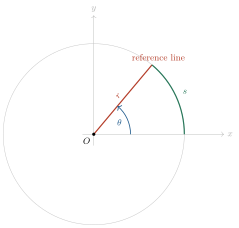
\includegraphics{figures/ch10/fig-1.pdf}
\caption{خاکہ 1: زاویائی مقام \hbox{$\theta$}، قوس \hbox{$s$} اور نصف قطر \hbox{$r$}۔
خطِ حوالہ مثبت \hbox{$x$} محور سے زاویہ \hbox{$\theta$} بناتا ہے۔}
\end{figure}

ریڈین دو لمبائیوں کا تناسب ہونے کے سبب ایک خالص عدد ہے اور بے اِبعاد ہے۔
چونکہ \(r\) نصف قطر والے دائرے کا محیط \(2\pi r\) ہوتا ہے، اِس لیے پورے
دائرے میں \(2\pi\) ریڈین ہوتے ہیں:

\[1\ \mathrm{rev} = 360^{\circ} = 2\pi\ \mathrm{rad}, \qquad 1\ \mathrm{rad} \approx 57.3^{\circ} \approx 0.159\ \mathrm{rev}.\]

\hypertarget{ux632ux627ux648ux6ccux627ux626ux6cc-ux627ux646ux62aux642ux627ux644}{%
\subsection{زاویائی
انتقال}\label{ux632ux627ux648ux6ccux627ux626ux6cc-ux627ux646ux62aux642ux627ux644}}

اگر جسم اپنا زاویائی مقام \(\theta_1\) سے \(\theta_2\) تک بدلے تو
\textbf{زاویائی انتقال} \en{(angular displacement)}:

\[\Delta\theta = \theta_2 - \theta_1.\]

اصول: گھڑی کی مخالف سمت میں گردش \textbf{مثبت} اور گھڑی کی سمت میں
\textbf{منفی} ہوتی ہے۔

\hypertarget{ux632ux627ux648ux6ccux627ux626ux6cc-ux631ux641ux62aux627ux631}{%
\subsection{زاویائی
رفتار}\label{ux632ux627ux648ux6ccux627ux626ux6cc-ux631ux641ux62aux627ux631}}

\(\Delta t\) وقفے میں \textbf{اوسط زاویائی رفتار}:

\[\omega_{\mathrm{avg}} = \frac{\theta_2-\theta_1}{t_2-t_1} = \frac{\Delta\theta}{\Delta t}.\]

\textbf{لمحاتی زاویائی رفتار} (\(\omega\)) اِسی تناسب کی وہ حد ہے جب
\(\Delta t \to 0\):

\[\omega = \frac{d\theta}{dt}.\]

اِس کی اکائی عموماً \(\mathrm{rad/s}\) ہوتی ہے۔

\hypertarget{ux632ux627ux648ux6ccux627ux626ux6cc-ux627ux633ux631ux627ux639}{%
\subsection{زاویائی
اسراع}\label{ux632ux627ux648ux6ccux627ux626ux6cc-ux627ux633ux631ux627ux639}}

اگر زاویائی رفتار \(\omega_1\) سے \(\omega_2\) تک بدلے تو \textbf{اوسط
زاویائی اسراع}:

\[\alpha_{\mathrm{avg}} = \frac{\omega_2-\omega_1}{t_2-t_1} = \frac{\Delta\omega}{\Delta t}, \qquad \alpha = \frac{d\omega}{dt}.\]

اکائی عموماً \(\mathrm{rad/s^2}\) ہوتی ہے۔

\hypertarget{ux6a9ux6ccux627-ux632ux627ux648ux6ccux627ux626ux6cc-ux645ux642ux62fux627ux631ux6ccux6ba-ux633ux645ux62aux6ccux6c1-ux6c1ux6ccux6ba}{%
\subsection{کیا زاویائی مقداریں سمتیہ
ہیں؟}\label{ux6a9ux6ccux627-ux632ux627ux648ux6ccux627ux626ux6cc-ux645ux642ux62fux627ux631ux6ccux6ba-ux633ux645ux62aux6ccux6c1-ux6c1ux6ccux6ba}}

زاویائی رفتار اور زاویائی اسراع کو \textbf{سمتیہ} \en{(vectors)} کے طور پر
دکھایا جا سکتا ہے: اِن کا رخ محورِ گردش کے ساتھ ساتھ ہوتا ہے، جسے
\textbf{دائیں ہاتھ کے اصول} سے طے کیا جاتا ہے۔

\begin{figure}
\centering
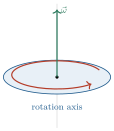
\includegraphics{figures/ch10/fig-2.pdf}
\caption{خاکہ 2: زاویائی رفتار کا سمتیہ \hbox{$\vec{\omega}$} محورِ گردش کے
ساتھ ہوتا ہے۔ دائیں ہاتھ کا اصول اِس کا رخ طے کرتا ہے۔}
\end{figure}

\hypertarget{ux645ux633ux62aux642ux644-ux632ux627ux648ux6ccux627ux626ux6cc-ux627ux633ux631ux627ux639-ux6a9ux6d2-ux633ux627ux62aux6be-ux6afux631ux62fux634}{%
\section{مستقل زاویائی اسراع کے ساتھ
گردش}\label{ux645ux633ux62aux642ux644-ux632ux627ux648ux6ccux627ux626ux6cc-ux627ux633ux631ux627ux639-ux6a9ux6d2-ux633ux627ux62aux6be-ux6afux631ux62fux634}}

جیسے انتقالی حرکت میں مستقل اسراع ایک اہم خاص صورت ہے، ویسے ہی گردش میں
\textbf{مستقل زاویائی اسراع} اہم ہے۔ حرکیاتی مساوات انتقالی مساوات کے
بالکل متوازی ہیں --- صرف \(x \to \theta\)، \(v \to \omega\)،
\(a \to \alpha\) رکھ دیں:

\[\begin{aligned}
\omega &= \omega_0 + \alpha t,\\
\theta - \theta_0 &= \omega_0 t + \tfrac{1}{2}\alpha t^2,\\
\omega^2 &= \omega_0^2 + 2\alpha(\theta-\theta_0).
\end{aligned}\]

\hypertarget{ux645ux62bux627ux644-1-ux645ux633ux62aux642ux644-ux632ux627ux648ux6ccux627ux626ux6cc-ux627ux633ux631ux627ux639}{%
\subsection{مثال 1: مستقل زاویائی
اسراع}\label{ux645ux62bux627ux644-1-ux645ux633ux62aux642ux644-ux632ux627ux648ux6ccux627ux626ux6cc-ux627ux633ux631ux627ux639}}

\textbf{سوال:} ایک پہیہ سکون سے شروع ہوتا ہے اور
\(\alpha = 2.0\ \mathrm{rad/s^2}\) کے مستقل اسراع سے گھومتا ہے۔
\(t = 5.0\ \mathrm{s}\) پر اِس کی زاویائی رفتار اور طے شدہ زاویہ کیا ہوں
گے؟

\textbf{حل:} چونکہ \(\omega_0 = 0\):

\[\omega = \omega_0 + \alpha t = (2.0)(5.0) = 10\ \mathrm{rad/s},\]

\[\theta - \theta_0 = \tfrac{1}{2}\alpha t^2 = \tfrac{1}{2}(2.0)(5.0)^2 = 25\ \mathrm{rad}.\]

\hypertarget{ux62eux637ux6cc-ux627ux648ux631-ux632ux627ux648ux6ccux627ux626ux6cc-ux645ux62aux63aux6ccux631ux627ux62a-ux6a9ux627-ux62aux639ux644ux642}{%
\section{خطی اور زاویائی متغیرات کا
تعلق}\label{ux62eux637ux6cc-ux627ux648ux631-ux632ux627ux648ux6ccux627ux626ux6cc-ux645ux62aux63aux6ccux631ux627ux62a-ux6a9ux627-ux62aux639ux644ux642}}

جب کوئی صلب جسم محور کے گرد گھومتا ہے تو اُس کا ہر نقطہ اپنے اپنے دائرے
میں گھومتا ہے۔ سب کی زاویائی رفتار \(\omega\) یکساں ہوتی ہے، مگر محور سے
جتنا دور نقطہ ہو، اُس کی \textbf{خطی رفتار} اُتنی زیادہ ہوتی ہے۔

\[s = \theta r, \qquad v = \omega r, \qquad a_t = \alpha r, \qquad a_r = \frac{v^2}{r} = \omega^2 r.\]

\begin{figure}
\centering
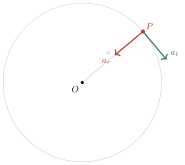
\includegraphics{figures/ch10/fig-3.pdf}
\caption{خاکہ 3: گھومتے جسم کے نقطہ \hbox{$P$} پر خطی اسراع کے دو اجزا ---
مماسی \hbox{$a_t = \alpha r$} اور نصف قطری \hbox{$a_r = \omega^2 r$}۔}
\end{figure}

\hypertarget{ux6afux631ux62fux634ux6cc-ux62cux645ux648ux62f-ux627ux648ux631-ux645ux62aux648ux627ux632ux6cc-ux645ux62dux648ux631-ux6a9ux627-ux645ux633ux626ux644ux6c1}{%
\section{گردشی جمود اور متوازی محور کا
مسئلہ}\label{ux6afux631ux62fux634ux6cc-ux62cux645ux648ux62f-ux627ux648ux631-ux645ux62aux648ux627ux632ux6cc-ux645ux62dux648ux631-ux6a9ux627-ux645ux633ux626ux644ux6c1}}

گھومتے جسم کی کل حرکی توانائی:

\[K = \tfrac{1}{2} I \omega^2, \qquad I = \sum m_i r_i^2 = \int r^2\, dm.\]

اگر مرکزِ کمیت سے گزرتے محور کے گرد جمود \(I_{\mathrm{com}}\) معلوم ہو، تو
\(h\) فاصلے پر متوازی محور کے گرد:

\[I = I_{\mathrm{com}} + M h^2\]

(متوازی محور کا مسئلہ)

\begin{figure}
\centering
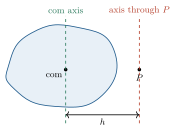
\includegraphics{figures/ch10/fig-4.pdf}
\caption{خاکہ 4: متوازی محور کا مسئلہ --- مرکزِ کمیت سے گزرتے محور اور
\hbox{$P$} سے گزرتے متوازی محور کے درمیان فاصلہ \hbox{$h$}۔}
\end{figure}

\hypertarget{ux645ux631ux648ux691}{%
\section{مروڑ}\label{ux645ux631ux648ux691}}

\textbf{مروڑ} \en{(torque)} کسی جسم پر، کسی محور کے گرد، قوت کے ذریعے پیدا
ہونے والا گھمانے کا عمل ہے۔ مروڑ کی مقدار:

\[\tau = r F \sin\phi = r_\perp F,\]

جہاں \(r_\perp = r\sin\phi\) \textbf{بازوئے مروڑ} \en{(moment arm)} --- محور
سے قوت کے خطِ عمل تک عمودی فاصلہ --- ہے۔

\begin{figure}
\centering
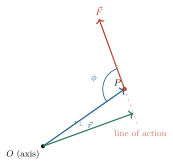
\includegraphics{figures/ch10/fig-5.pdf}
\caption{خاکہ 5: مروڑ \hbox{$\tau = rF\sin\phi$}۔ \hbox{$\vec{r}$} مقام سمتیہ،
\hbox{$\vec{F}$} قوت، \hbox{$\phi$} اُن کے درمیان زاویہ، اور \hbox{$r_\perp$} بازوئے
مروڑ۔}
\end{figure}

گردش کے لیے نیوٹن کا دوسرا قانون:

\[\tau_{\mathrm{net}} = I\alpha\]

(ریڈین میں)

\hypertarget{ux62eux644ux627ux635ux6c1}{%
\section*{خلاصہ}\label{ux62eux644ux627ux635ux6c1}}
\addcontentsline{toc}{section}{خلاصہ}

\textbf{گردشی متغیرات:} \(\theta = s/r\)؛ \(\omega = d\theta/dt\)؛
\(\alpha = d\omega/dt\)۔ گھڑی کی مخالف سمت مثبت۔

\textbf{خطی--زاویائی تعلق:} \(s = \theta r\)، \(v = \omega r\)،
\(a_t = \alpha r\)، \(a_r = \omega^2 r\)۔

\textbf{گردشی جمود اور توانائی:} \(K = \tfrac{1}{2}I\omega^2\)؛ متوازی
محور: \(I = I_{\mathrm{com}} + Mh^2\)۔

\textbf{مروڑ:} \(\tau = rF\sin\phi = r_\perp F\)؛ گردش کا نیوٹن دوسرا
قانون: \(\tau_{\mathrm{net}} = I\alpha\)۔

\clearpage
\end{document}